\documentclass{article}

\usepackage{amsmath}
\usepackage[usenames,dvipsnames]{color}
\usepackage{multirow}
\usepackage{listings}
\usepackage[a4paper, top=2cm, bottom=3cm, left=4cm, right=4cm]{geometry}

\usepackage{tikz}
\usetikzlibrary{shapes, shapes.multipart, shapes.geometric}
\usetikzlibrary{positioning}

\newcommand*\circled[1]{\tikz[baseline=(char.base)]{
    \node[shape=circle,draw,inner sep=2pt] (char) {#1};}}

\newcommand{\bfc}{{\sc Bfc}}
\newcommand{\mist}{{\sc Mist}}
\newcommand{\pnerf}{{\sc Pnerf}}
\newcommand{\zthree}{{\sc Z3}}
\newcommand{\ttt}[1]{\texttt{#1}}

\begin{document}


\title{Experimental Results \\ \mbox{ } \\ of a Safety Checker for Petri nets}
\author{Philipp Meyer \and Rusl\'{a}n Ledesma-Garza}
% \institute{Technische Universit\"at M\"unchen}
\date{\today}

\maketitle

We report on the experimental results of a constraint based
approach for checking safety of Petri Nets.
We implemented the approach in the tool \pnerf. \pnerf\ abstracts a
given Petri Net as a set of state constraints over integers or
reals. When state constraints are not sufficient for checking safety,
\pnerf\ refines the abstraction by applying three techniques (i.e. TrapConditions,
SubnetTrapConditions, EmptyTrapConditions). Each technique constructs additional
state constraints from the spurious abstract
counterexample (i.e. the valuation corresponding state constraints) when possible.
We applied \zthree\ as the backend.
As an experiment, we substituted the refinement techniques with
concrete concrete state exploration. We also report on the
corresponding results.


\section{Benchmarks of \bfc}

We experimented on the benchmarks \ttt{cprover-PN} and
\ttt{cprover\_software\_analysis}
available at
\ttt{http://www.mpi-sws.org/\~{}jkloos/iic-experiments/cprover.zip}.
The set of benchmarks consists 77 benchmarks, 26 positive and 51 negative.
We applied 8 tool configurations to the set of benchmarks.
Table~\ref{bfc-experiments} shows the corresponding experimental results.

\begin{table}[h]
\begin{center}
  \begin{tabular}{ | r | p{7cm} | r | r | r | r | } %
    \hline
    \multicolumn{2}{|l|}{Configuration} & pos & neg & don't know & TO \\
    \hline
    C1 & State constraint over real numbers & 23 &  0 & 54 &  0 \\
    C2 & State constraint over integers        & 23 &  0 & 54 &  0 \\
    \hline
    C3 & C2 + TrapConditions                   & 23 &  0 & 54 &  0 \\
    C4 & C3 + SubnetTrapConditions         & 23 &  0 & 50 &  4 \\
    C5 & C4 + EmptyTrapConditions          & 23 &  0 & 46 &  8 \\
    \hline
    C6 & C1 + state space exploration \& TO 1\,min & 26 & 34 & 0 & 17 \\
    C7 & C1 + state space exploration \& TO 10\,min & 26 & 39 & 0 & 12 \\
    C8 & C1 + state space exploration \& TO 8\,h   & 26 & 45 & 0 &  6 \\
    \hline
  \end{tabular}
\end{center}
\caption{Experimental results for the benchmarks of \bfc}
\label{bfc-experiments}
\end{table}

Observations:
\begin{itemize}
\item State constraints over integers or reals correctly determine that the 23 benchmarks in Appendix~\ref{bfc-experiments-c1} are positive.
\item Composing state space constraints with concrete state space
  exploration gives the following 3 additional positives.
\begin{verbatim}
cprover-PN/lamport
cprover-PN/newdekker
cprover-PN/peterson
\end{verbatim}
\end{itemize}


\newpage

\section{Benchmarks of \mist}

We experimented on the benchmarks available at \\
\ttt{https://github.com/pierreganty/mist/tree/master/examples/boundedPN}
and \\
\ttt{https://github.com/pierreganty/mist/tree/master/examples/PN}.
The set of benchmarks consists 27 benchmarks, 23 positive and 4 negative.
We applied 6 tool configurations to the set of benchmarks.
Table~\ref{mist-experiments} shows the corresponding experimental results.

\begin{table}[h]
\begin{center}
  \begin{tabular}{ | r | p{6cm} | r | r | r | r | }
    \hline
    \multicolumn{2}{|l|}{Configuration} & pos & neg & don't know & TO \\
    \hline
    C1 & State constraint with real numbers & 14 &  0 & 13 &  0 \\
    C2 & State constraint with integers     & 14 &  0 & 13 &  0 \\
    \hline
    C3 & C2 + TrapConditions               & 20 &  0 &  7 &  0 \\
    C4 & C3 + SubnetTrapConditions         & 21 &  0 &  6 &  0 \\
    C5 & C4 + EmptyTrapConditions          & 21 &  0 &  6 &  0 \\
    \hline
    C9 & C4 + state space exploration \& TO 4\,h & 21 &  2 & 0 &  4 \\
    \hline
  \end{tabular}
\end{center}
\caption{Experimental results for the benchmarks of \mist}
\label{mist-experiments}
\end{table}

Observations:
\begin{itemize}
\item State constraints over integers or reals correctly determine that the 14 benchmarks in Appendix~\ref{mist-experiments-c1} are positive.
\item Composing state constraints with TrapConditions gives the following 6 additional positives.
\begin{verbatim}
PN/pingpong
PN/basicME
PN/multiME
boundedPN/lamport
boundedPN/newdekker
boundedPN/peterson
\end{verbatim}
\item Composing state constraints with TrapConditions and SubnetTrapConditions gives the additional positive \ttt{PN/manufacturing}.
  \item The remaining positive benchmarks are the following.
\begin{verbatim}
PN/extendedread-write
PN/extendedread-write-smallconsts
\end{verbatim}
\end{itemize}

\newpage

\iffalse
\section{Method}

\begin{figure}[ht]
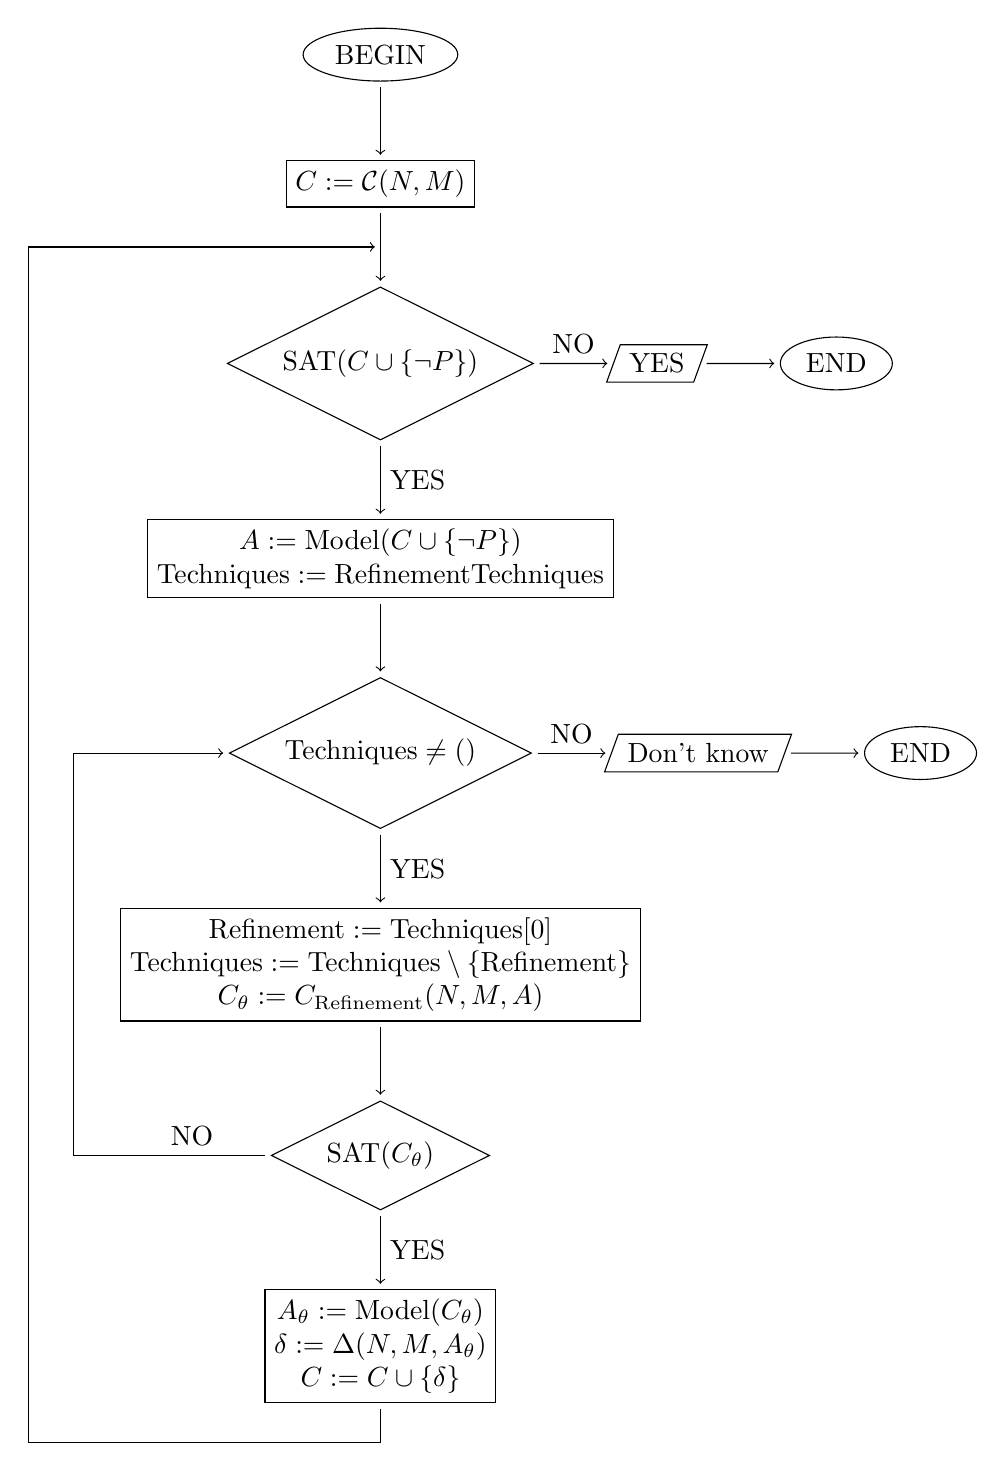
\begin{tikzpicture}[
    state/.style   = {draw, ellipse, aspect=2},
    action/.style  = {draw, rectangle, align=center},
    decision/.style= {draw, diamond, aspect=2, align=center},
    print/.style   = {draw, trapezium, trapezium left angle=70, trapezium right angle=-70},
    edge/.style    = {draw, ->, shorten >=2pt, shorten <=2pt},
  ]
  \node[state] (begin) {BEGIN};
  \node[action, below=of begin] (c) {$C:=\mathcal C(N, M)$};
  \node[decision, below=of c] (satc) {$\text{SAT}(C \cup \{\neg P\})$};
  \node[action, below=of satc] (modelc)
    {$A:=\text{Model}(C \cup \{\neg P\})$ \\
     $\text{Techniques}:=\text{RefinementTechniques}$};
     \node[decision, below=of modelc] (methods) {$\text{Techniques} \neq ()$};
  \node[action, below=of methods] (ctheta)
    {$\text{Refinement} := \text{Techniques}[0]$ \\
     $\text{Techniques}:= \text{Techniques} \setminus \{\text{Refinement}\}$ \\
     $C_{\theta}:=C_{\text{Refinement}}(N, M, A)$};
  \node[decision, below=of ctheta] (satctheta) {$\text{SAT}(C_\theta)$};
  \node[action, below=of satctheta] (modelctheta)
    {$A_\theta:=\text{Model}(C_\theta)$\\
     $\delta:=\Delta(N, M, A_\theta)$\\
     $C:=C \cup \{\delta\}$};
  \node[print, right=of satc] (yes) {YES};
  \node[state, right=of yes] (end1) {END};
  \node[print, right=of methods] (dontknow) {Don't know};
  \node[state, right=of dontknow] (end2) {END};

  \draw (begin) edge[edge] (c);
  \draw (c) edge[edge] coordinate[pos=.5] (edgein) (satc);
  \draw (satc) edge[edge] node[above]{NO} (yes);
  \draw (yes) edge[edge] (end1);
  \draw (satc) edge[edge] node[right]{YES} (modelc);
  \draw (modelc) edge[edge] (methods);
  \draw (methods) edge[edge] node[right]{YES}  (ctheta);
  \draw (methods) edge[edge] node[above]{NO} (dontknow);
  \draw (ctheta) edge[edge] (satctheta);
  \draw (dontknow) edge[edge] (end2);
  \draw (satctheta) edge[edge] node[right]{YES} (modelctheta);
  \draw[edge] (satctheta.west) node[above,xshift=-1cm]{NO}
  -| ([xshift=-2.5cm] satctheta.west) |- (methods.west);
  \draw[edge] (modelctheta.south) -- ([yshift=-0.5cm] modelctheta.south)
  -| ([xshift=-3cm] modelctheta.west) |- (edgein);
\end{tikzpicture}
\caption{The method}
\label{fig-method}
\end{figure}
\fi

\section*{Appendix}

\subsection{Benchmarks for Table~\ref{bfc-experiments}, configuration C1}
\label{bfc-experiments-c1}

\begin{verbatim}
cprover-PN/abp
cprover-PN/basicME
cprover-PN/bingham_h150
cprover-PN/bingham_h25
cprover-PN/bingham_h250
cprover-PN/bingham_h50
cprover-PN/bingham_h500
cprover-PN/clientserver
cprover-PN/csm
cprover-PN/gsm
cprover-PN/handover
cprover-PN/keycard
cprover-PN/mesh2x2
cprover-PN/multipoll
cprover-PN/newrtp
cprover-PN/phones
cprover-PN/reaction
cprover-PN/reaction3
cprover-PN/reaction4
cprover-PN/read-write
cprover-PN/restriction
cprover_software_analysis/conditionals_vs_satabs.2/main
cprover_software_analysis/rand_cas_vs_satabs.2/main
\end{verbatim}




\subsection{Benchmarks for Table~\ref{mist-experiments}, configuration C1}
\label{mist-experiments-c1}

\begin{verbatim}
PN/MultiME
PN/basicME
PN/bingham_h150
PN/bingham_h25
PN/bingham_h250
PN/bingham_h250_attic
PN/bingham_h50
PN/csm
PN/fms
PN/fms_attic
PN/mesh2x2
PN/mesh3x2
PN/multipool
boundedPN/kanban
boundedPN/newrtp
boundedPN/read-write
\end{verbatim}







\end{document}
